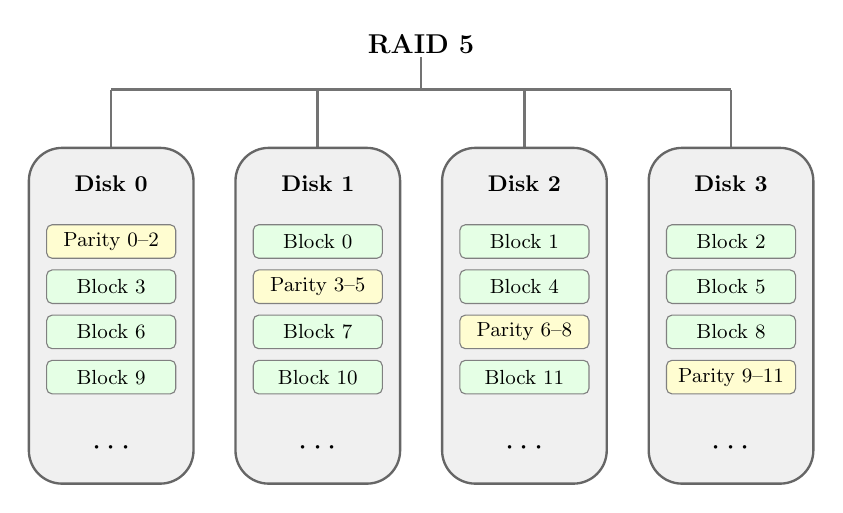
\begin{tikzpicture}[
    x=1cm,y=1cm,
    scale=0.82,
    transform shape,
    every node/.style={font=\small},
    frame/.style={draw=black!60, rounded corners=12pt, line width=0.85pt},
    drive/.style={frame, fill=gray!12, minimum width=2.55cm, minimum height=5.20cm},
    block/.style={draw=black!50, rounded corners=2pt, fill=green!10, minimum width=2.0cm, minimum height=0.52cm},
    parity/.style={draw=black!50, rounded corners=2pt, fill=yellow!18, minimum width=2.0cm, minimum height=0.52cm},
    bracket/.style={draw=black!55, line width=0.95pt}
]
    \node[font=\bfseries\large] (title) at (4.8,4.20) {RAID 5};
    \draw[bracket] (0,3.50) -- (9.6,3.50);
    \foreach \x in {0,3.2,6.4,9.6} {
        \draw[bracket] (\x,2.60) -- (\x,3.50);
    }
    \draw[bracket] (4.8,3.50) -- (4.8,4.00);

    \foreach \x/\name in {0/Disk 0,3.2/Disk 1,6.4/Disk 2,9.6/Disk 3} {
        \node[drive] at (\x,0) {};
        \node[font=\bfseries] at (\x,2.05) {\name};
        \node[font=\Large] at (\x,-2.05) {$\cdots$};
    }

    \node[parity] at (0,1.15) {Parity 0--2};
    \node[block] at (3.2,1.15) {Block 0};
    \node[block] at (6.4,1.15) {Block 1};
    \node[block] at (9.6,1.15) {Block 2};

    \node[block] at (0,0.45) {Block 3};
    \node[parity] at (3.2,0.45) {Parity 3--5};
    \node[block] at (6.4,0.45) {Block 4};
    \node[block] at (9.6,0.45) {Block 5};

    \node[block] at (0,-0.25) {Block 6};
    \node[block] at (3.2,-0.25) {Block 7};
    \node[parity] at (6.4,-0.25) {Parity 6--8};
    \node[block] at (9.6,-0.25) {Block 8};

    \node[block] at (0,-0.95) {Block 9};
    \node[block] at (3.2,-0.95) {Block 10};
    \node[block] at (6.4,-0.95) {Block 11};
    \node[parity] at (9.6,-0.95) {Parity 9--11};
\end{tikzpicture}